We demonstrate the system using three representative workflows.

Each workflow produces structured outputs including statistical tables and formatted figures. Figure~\ref{fig:gallery} shows representative outputs from the literature review, biomarker discovery, and causal inference pipelines.

\begin{figure}[h]
    \centering
    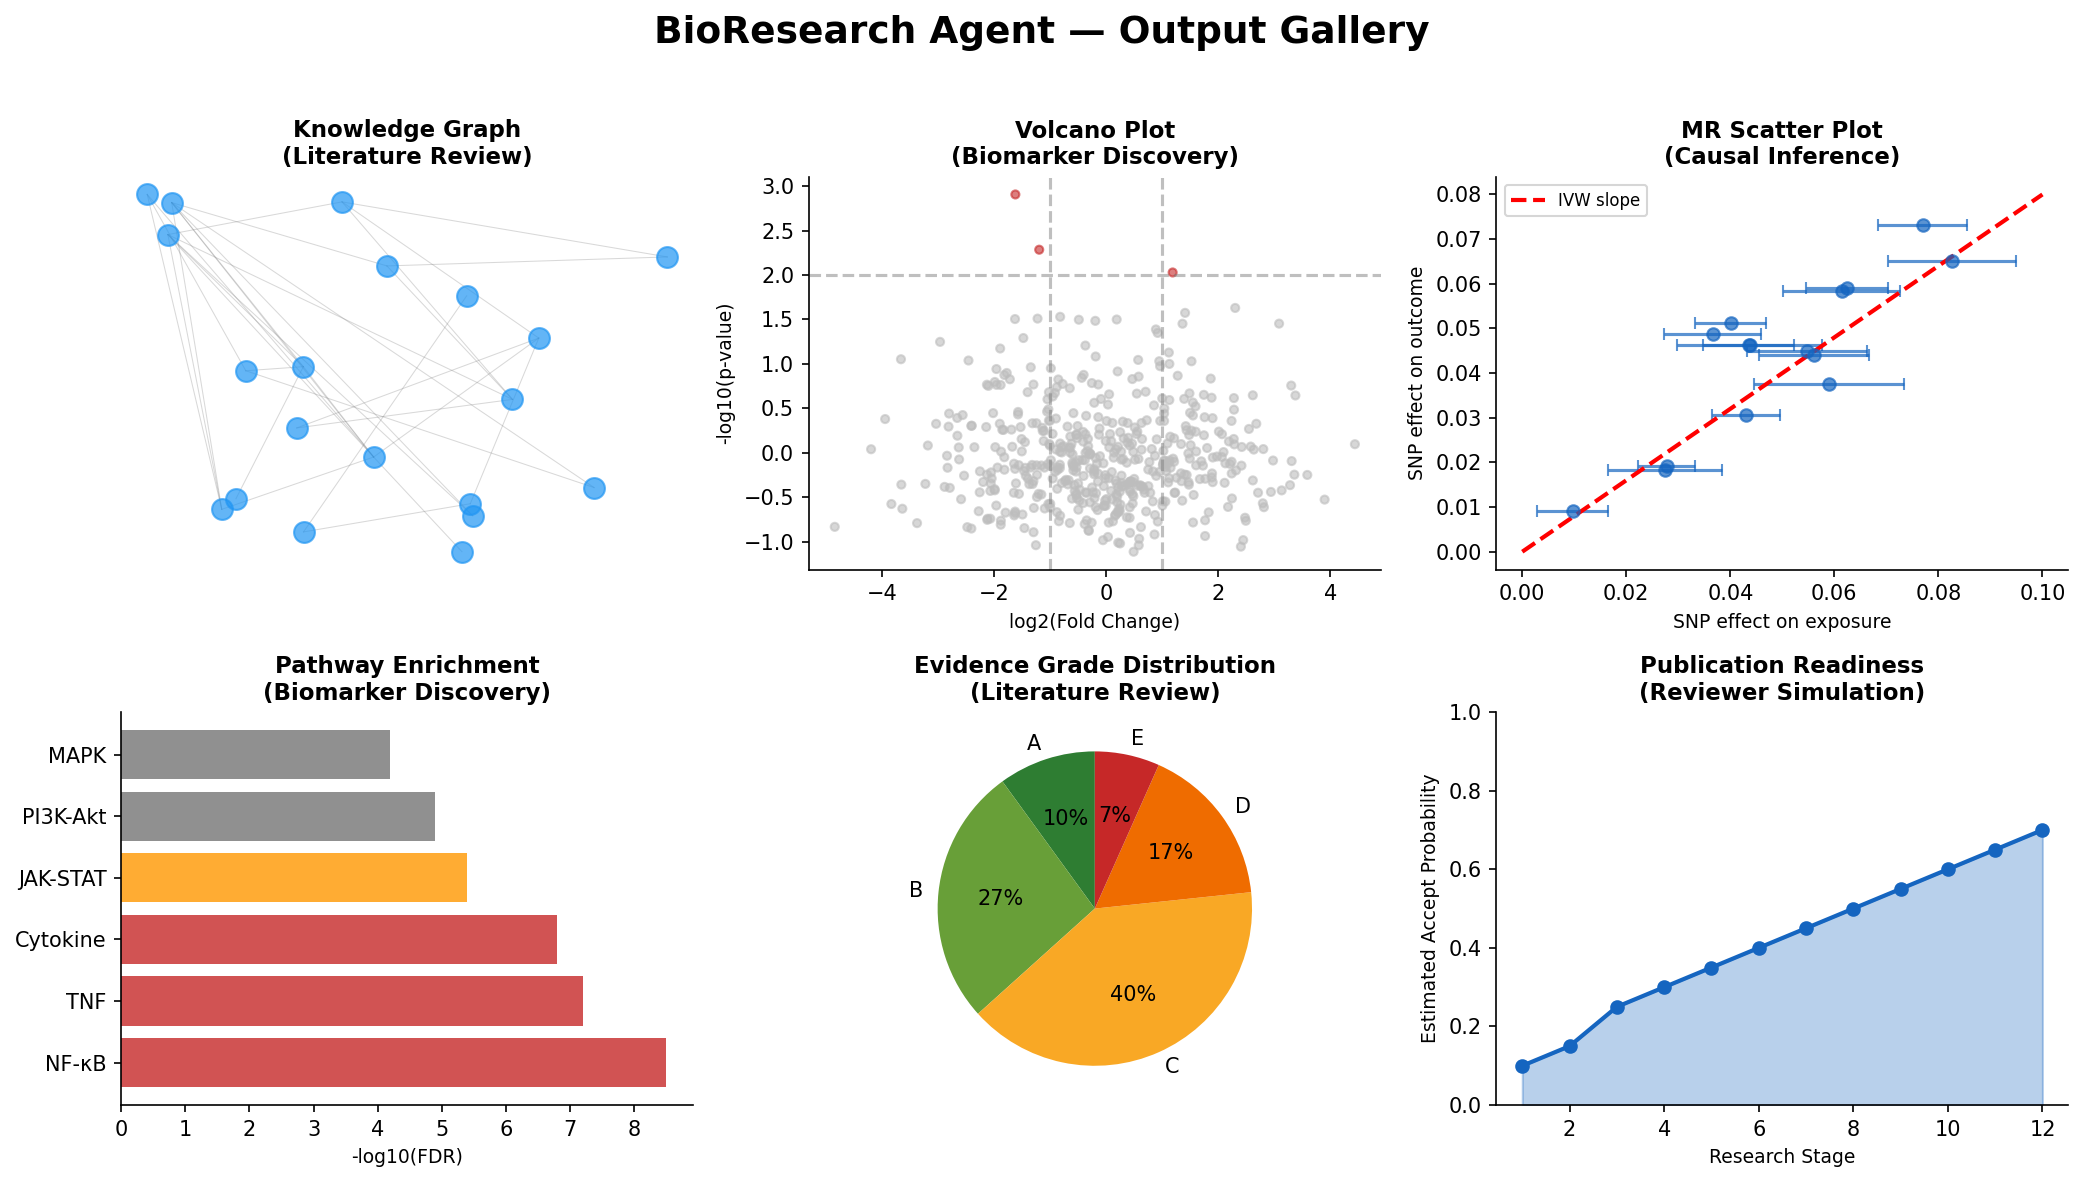
\includegraphics[width=0.9\linewidth]{figures/fig3_output_gallery}
    \caption{Representative outputs from three analysis pipelines: literature co-occurrence graph, differential-expression volcano plot, and Mendelian-randomization scatter and funnel plots.}
    \label{fig:gallery}
\end{figure}

Figure~\ref{fig:execution} shows the twelve-stage execution diagram that maps the typical biomedical research workflow from question formulation to formatted output. Stages 1--8 are implemented in the current release; stages 9--12 (writing, review, critique, formatted output) represent conceptual extensions of the end-to-end workflow and are not automated in the current system.

\begin{figure}[h]
    \centering
    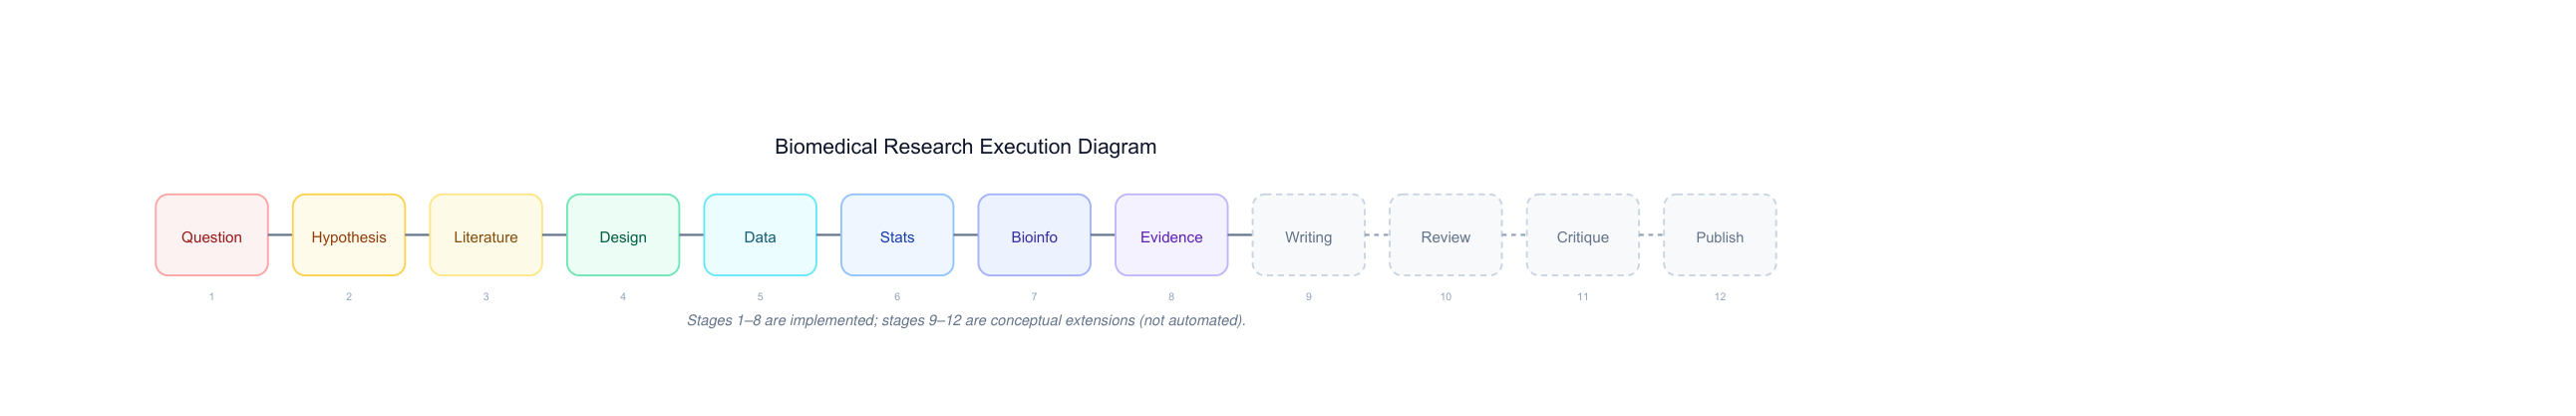
\includegraphics[width=0.9\linewidth]{figures/fig2_execution}
    \caption{Execution diagram across 12 stages. Stages 1--8 are implemented in the current release; stages 9--12 represent conceptual extensions and are not automated.}
    \label{fig:execution}
\end{figure}